\documentclass{standalone}
\usepackage{tikz,tikz-3dplot}
\usetikzlibrary{perspective,patterns}
\usetikzlibrary{calc,fadings,decorations.pathreplacing}
\usetikzlibrary{shapes,fit}
\usetikzlibrary{hobby}
\usetikzlibrary{arrows.meta}
\begin{document}
\tikzset{illustration/.style={very thin}}
\tikzset{dimension/.style={very thin,lightgray}}
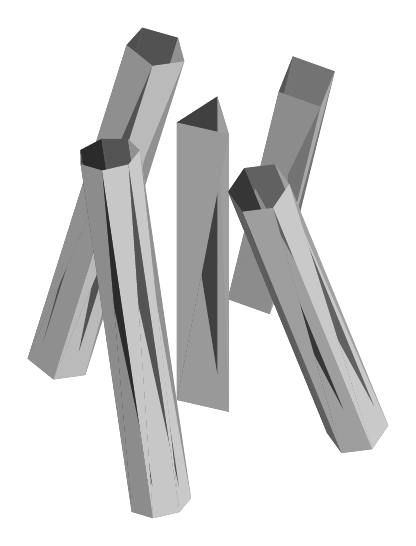
\begin{tikzpicture}[3d view={17.761769326897024}{45.18699125315629},fill=gray]
\fill (0.3464,-0.2)--(-0.3464,-0.2)--(0,0.4)--cycle;
\fill (0,0.4,5.0)--(-0.3464,-0.2,5.0)--(0.3464,-0.2,5.0)--cycle;
\fill (-1.8286,0.3462,-0.1035)--(-1.6112,-0.0688,-0.064)--(-1.9312,-0.3888,0.064)--(-2.3462,-0.1714,0.1035)--(-2.2828,0.2828)--cycle;
\fill (-1.2828,1.2828,5.0)--(-1.3462,0.8286,5.1035)--(-0.9312,0.6112,5.064)--(-0.6112,0.9312,4.936)--(-0.8286,1.3462,4.8965)--cycle;
\fill (0.2722,1.7278,-0.1089)--(-0.2828,1.7172,0)--(-0.2722,2.2722,0.1089)--(0.2828,2.2828)--cycle;
\fill (1.2828,1.2828,5.0)--(0.7278,1.2722,5.1089)--(0.7172,0.7172,5.0)--(1.2722,0.7278,4.8911)--cycle;
\fill (1.9057,-0.3771,-0.0943)--(1.6229,-0.0943,-0.0943)--(1.7172,0.2828,0)--(2.0943,0.3771,0.0943)--(2.3771,0.0943,0.0943)--(2.2828,-0.2828)--cycle;
\fill (1.2828,-1.2828,5.0)--(1.3771,-0.9057,5.0943)--(1.0943,-0.6229,5.0943)--(0.7172,-0.7172,5.0)--(0.6229,-1.0943,4.9057)--(0.9057,-1.3771,4.9057)--cycle;
\fill (-0.3891,-1.9636,-0.0851)--(-0.2024,-1.6717,-0.1061)--(0.1367,-1.6271,-0.0472)--(0.3729,-1.8633,0.0472)--(0.3283,-2.2024,0.1061)--(0.0364,-2.3891,0.0851)--(-0.2828,-2.2828)--cycle;
\fill (-1.2828,-1.2828,5.0)--(-0.9636,-1.3891,5.0851)--(-0.6717,-1.2024,5.1061)--(-0.6271,-0.8633,5.0472)--(-0.8633,-0.6271,4.9528)--(-1.2024,-0.6717,4.8939)--(-1.3891,-0.9636,4.9149)--cycle;
\fill[white!45!black] (0.2828,2.2828,0.0)--(-0.2722,2.2722,0.1089)--(0.7278,1.2722,5.1089)--cycle;
\fill[white!66!black] (0.2722,1.7278,-0.1089)--(0.2828,2.2828,0.0)--(1.2828,1.2828,5.0)--cycle;
\fill[white!34!black] (-0.2722,2.2722,0.1089)--(-0.2828,1.7172,0)--(0.7172,0.7172,5.0)--cycle;
\fill[white!55!black] (-0.2828,1.7172,0)--(0.2722,1.7278,-0.1089)--(1.2722,0.7278,4.8911)--cycle;
\fill[white!32!black] (-1.8286,0.3462,-0.1035)--(-2.2828,0.2828,0.0)--(-1.2828,1.2828,5.0)--cycle;
\fill[white!57!black] (-1.6112,-0.0688,-0.064)--(-1.8286,0.3462,-0.1035)--(-0.8286,1.3462,4.8965)--cycle;
\fill[white!31!black] (-2.2828,0.2828,0.0)--(-2.3462,-0.1714,0.1035)--(-1.3462,0.8286,5.1035)--cycle;
\fill[white!73!black] (-1.9312,-0.3888,0.064)--(-1.6112,-0.0688,-0.064)--(-0.6112,0.9312,4.936)--cycle;
\fill[white!56!black] (-2.3462,-0.1714,0.1035)--(-1.9312,-0.3888,0.064)--(-0.9312,0.6112,5.064)--cycle;
\fill[white!62!black] (0.3464,-0.2,0.0)--(0,0.4,0.0)--(0,0.4,5.0)--cycle;
\fill[white!25!black] (0,0.4,0.0)--(-0.3464,-0.2,0.0)--(-0.3464,-0.2,5.0)--cycle;
\fill[white!32!black] (-1.8286,0.3462,-0.1035)--(-1.2828,1.2828,5.0)--(-0.8286,1.3462,4.8965)--cycle;
\fill[white!45!black] (0.2828,2.2828,0.0)--(0.7278,1.2722,5.1089)--(1.2828,1.2828,5.0)--cycle;
\fill[white!60!black] (-0.3464,-0.2,0.0)--(0.3464,-0.2,0.0)--(0.3464,-0.2,5.0)--cycle;
\fill[white!31!black] (-2.2828,0.2828,0.0)--(-1.3462,0.8286,5.1035)--(-1.2828,1.2828,5.0)--cycle;
\fill[white!34!black] (-0.2722,2.2722,0.1089)--(0.7172,0.7172,5.0)--(0.7278,1.2722,5.1089)--cycle;
\fill[white!38!black] (2.0943,0.3771,0.0943)--(1.7172,0.2828,0)--(0.7172,-0.7172,5.0)--cycle;
\fill[white!21!black] (1.7172,0.2828,0)--(1.6229,-0.0943,-0.0943)--(0.6229,-1.0943,4.9057)--cycle;
\fill[white!63!black] (2.3771,0.0943,0.0943)--(2.0943,0.3771,0.0943)--(1.0943,-0.6229,5.0943)--cycle;
\fill[white!57!black] (-1.6112,-0.0688,-0.064)--(-0.8286,1.3462,4.8965)--(-0.6112,0.9312,4.936)--cycle;
\fill[white!66!black] (0.2722,1.7278,-0.1089)--(1.2828,1.2828,5.0)--(1.2722,0.7278,4.8911)--cycle;
\fill[white!55!black] (-0.2828,1.7172,0)--(1.2722,0.7278,4.8911)--(0.7172,0.7172,5.0)--cycle;
\fill[white!37!black] (1.6229,-0.0943,-0.0943)--(1.9057,-0.3771,-0.0943)--(0.9057,-1.3771,4.9057)--cycle;
\fill[white!56!black] (-2.3462,-0.1714,0.1035)--(-0.9312,0.6112,5.064)--(-1.3462,0.8286,5.1035)--cycle;
\fill[white!79!black] (2.2828,-0.2828,0.0)--(2.3771,0.0943,0.0943)--(1.3771,-0.9057,5.0943)--cycle;
\fill[white!73!black] (-1.9312,-0.3888,0.064)--(-0.6112,0.9312,4.936)--(-0.9312,0.6112,5.064)--cycle;
\fill[white!62!black] (1.9057,-0.3771,-0.0943)--(2.2828,-0.2828,0.0)--(1.2828,-1.2828,5.0)--cycle;
\fill[white!33!black] (0.1367,-1.6271,-0.0472)--(-0.2024,-1.6717,-0.1061)--(-1.2024,-0.6717,4.8939)--cycle;
\fill[white!17!black] (-0.2024,-1.6717,-0.1061)--(-0.3891,-1.9636,-0.0851)--(-1.3891,-0.9636,4.9149)--cycle;
\fill[white!57!black] (0.3729,-1.8633,0.0472)--(0.1367,-1.6271,-0.0472)--(-0.8633,-0.6271,4.9528)--cycle;
\fill[white!31!black] (-0.3891,-1.9636,-0.0851)--(-0.2828,-2.2828,0.0)--(-1.2828,-1.2828,5.0)--cycle;
\fill[white!25!black] (0,0.4,0.0)--(-0.3464,-0.2,5.0)--(0,0.4,5.0)--cycle;
\fill[white!79!black] (0.3283,-2.2024,0.1061)--(0.3729,-1.8633,0.0472)--(-0.6271,-0.8633,5.0472)--cycle;
\fill[white!62!black] (0.3464,-0.2,0.0)--(0,0.4,5.0)--(0.3464,-0.2,5.0)--cycle;
\fill[white!55!black] (-0.2828,-2.2828,0.0)--(0.0364,-2.3891,0.0851)--(-0.9636,-1.3891,5.0851)--cycle;
\fill[white!78!black] (0.0364,-2.3891,0.0851)--(0.3283,-2.2024,0.1061)--(-0.6717,-1.2024,5.1061)--cycle;
\fill[white!60!black] (-0.3464,-0.2,0.0)--(0.3464,-0.2,5.0)--(-0.3464,-0.2,5.0)--cycle;
\fill[white!17!black] (-0.2024,-1.6717,-0.1061)--(-1.3891,-0.9636,4.9149)--(-1.2024,-0.6717,4.8939)--cycle;
\fill[white!33!black] (0.1367,-1.6271,-0.0472)--(-1.2024,-0.6717,4.8939)--(-0.8633,-0.6271,4.9528)--cycle;
\fill[white!38!black] (2.0943,0.3771,0.0943)--(0.7172,-0.7172,5.0)--(1.0943,-0.6229,5.0943)--cycle;
\fill[white!21!black] (1.7172,0.2828,0)--(0.6229,-1.0943,4.9057)--(0.7172,-0.7172,5.0)--cycle;
\fill[white!63!black] (2.3771,0.0943,0.0943)--(1.0943,-0.6229,5.0943)--(1.3771,-0.9057,5.0943)--cycle;
\fill[white!31!black] (-0.3891,-1.9636,-0.0851)--(-1.2828,-1.2828,5.0)--(-1.3891,-0.9636,4.9149)--cycle;
\fill[white!57!black] (0.3729,-1.8633,0.0472)--(-0.8633,-0.6271,4.9528)--(-0.6271,-0.8633,5.0472)--cycle;
\fill[white!37!black] (1.6229,-0.0943,-0.0943)--(0.9057,-1.3771,4.9057)--(0.6229,-1.0943,4.9057)--cycle;
\fill[white!79!black] (2.2828,-0.2828,0.0)--(1.3771,-0.9057,5.0943)--(1.2828,-1.2828,5.0)--cycle;
\fill[white!62!black] (1.9057,-0.3771,-0.0943)--(1.2828,-1.2828,5.0)--(0.9057,-1.3771,4.9057)--cycle;
\fill[white!55!black] (-0.2828,-2.2828,0.0)--(-0.9636,-1.3891,5.0851)--(-1.2828,-1.2828,5.0)--cycle;
\fill[white!79!black] (0.3283,-2.2024,0.1061)--(-0.6271,-0.8633,5.0472)--(-0.6717,-1.2024,5.1061)--cycle;
\fill[white!78!black] (0.0364,-2.3891,0.0851)--(-0.6717,-1.2024,5.1061)--(-0.9636,-1.3891,5.0851)--cycle;
\end{tikzpicture}
\end{document}
